\section{The Higgs boson}
A lot of material here is for your benefit (the latter parts drawing heavily from Leonard Susskind's Stanford Lectures). Ultimately what I want you to understand is how the Higgs couples to the $W$, the $Z$ and fermions, what determines the coupling strength and what the experimental techniques are that led to its discovery and the subsequent measurements.

What you need to know is that:
{\bf The coupling strength of the Higgs boson to other particles, is proportional to the mass of the particle the Higgs couples to. So the probability that a Higgs will decay to a particular particle is proportional to the mass of the particle the Higgs couples to squared.}
Recent measurements seem to verify this fact as the figure below suggests. The y-axis is the coupling strength, the x-axis is the mass of the particle the Higgs decayed to.
\begin{center}
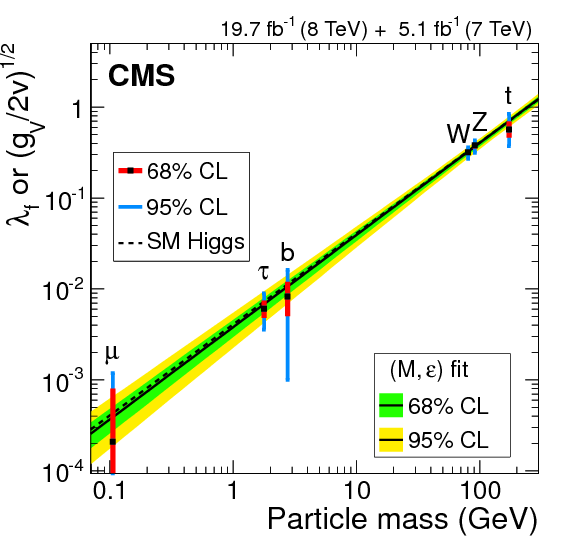
\includegraphics[width=0.95\textwidth]{fig/higgs/cms_higgs_couplings.png}
\end{center}

\exercise{
Given that measuring the Branching Fraction of the Higgs to a pair of $b$-quarks has been extremely challenging for experimentalists to measure, what are the prospects for measuring the Higgs couplings to a pair of strange quarks and why? (you can assume $m_s\sim100$MeV, $m_b\sim4$GeV)
}

So given the top quark is the heaviest of particles, they have the largest coupling strength. But we also need to be able to conserve energy and momentum. Thus given that we know that the Higgs boson has a mass $\sim125$~GeV, an ``on-shell'' Higgs boson cannot decay into two ``on-shell'' top-quarks. 

You might have heard that the Higgs boson was discovered in its decay to a pair of photons. How could that be given that photons are massless? Well it can happen through a loop-process shown below.
\begin{center}
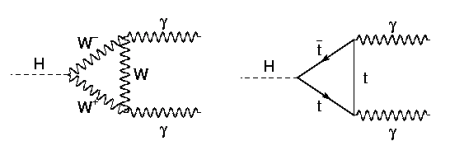
\includegraphics[width=0.95\textwidth]{fig/higgs/higgs_decay_photons.png}
\end{center}

\subsection{How do we produce a Higgs boson in experiments?}
\paragraph{pp-colliders}:
Note that strictly speaking the proton is not just made up of 3 quarks. Quantum mechanics as well as the confining nature of the strong force, allows for gluons to pop out of the vacuum and interact with the 3 valence quarks or split into quark anti-quark pairs. This is a whole separate topic we did not have enough time to cover.
So when colliding protons at high energies like at the LHC, what we are really colliding is primarily gluons within the proton as well as quark/anti-quarks.
\begin{center}
a)gluon-fusion, b) vector boson fusion, c) Higgs-strahlung (or associate production with W), d)associated production with tops
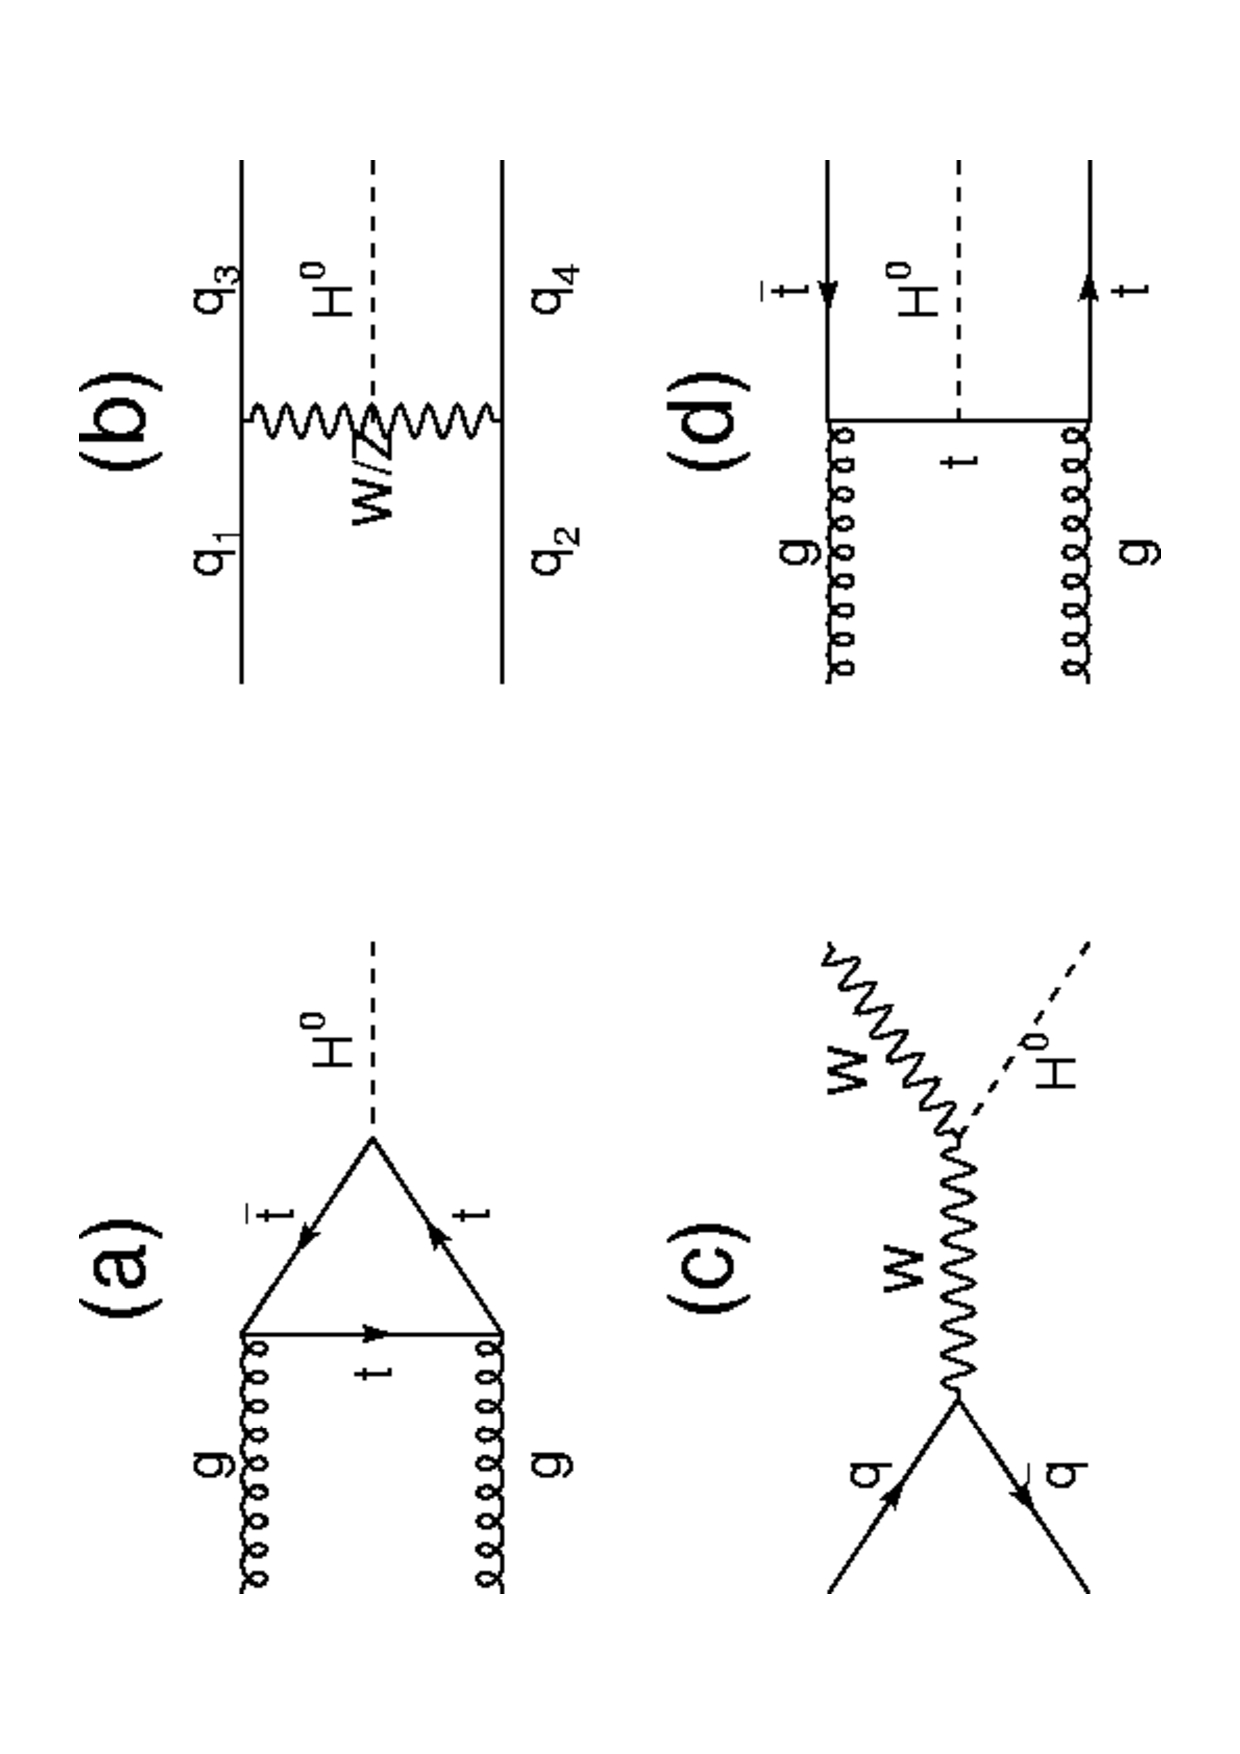
\includegraphics[angle=270,width=0.95\textwidth]{fig/higgs/higgs_production_lhc.pdf}
\end{center}

\paragraph{$e^+e^-$-colliders}:
If the collision energy is below $2\times m_{t}$ then the dominant production mechanism is via an off-shell $Z^0$ boson decaying to an on-shell $Z^0$ and a Higgs.
\begin{center}
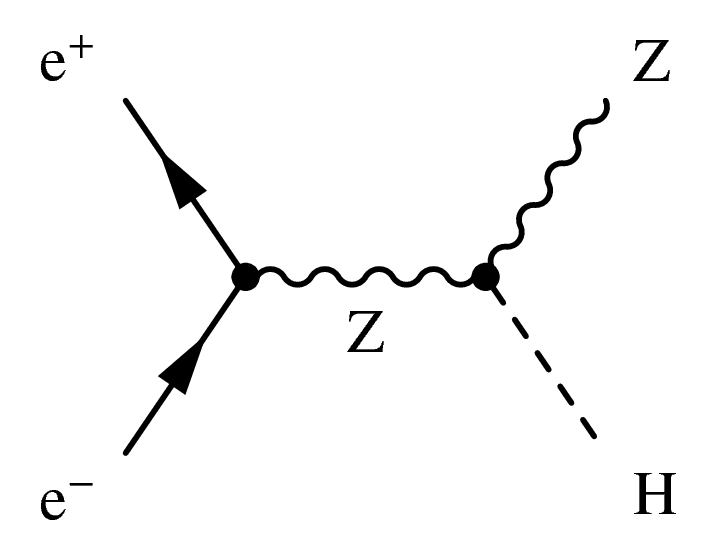
\includegraphics[width=0.55\textwidth]{fig/higgs/higgs_strahlung.png}
\end{center}
\exercise{
If the available CoM energy available in the $e^+e^-$ collision is $>2m_t$,
what do you think the dominant production mechanism of the Higgs could be?
}

A detailed discussion beyond the scope of the course on the proof of the Higgs mechanism
can be found in Appendix~\ref{sec:higgs_proof}.
